\subsubsection{ClientModel}

\textbf{GoIntentService}

\paragraph{Database}

\textbf{DBHelper}

Die vier nachfolgenden DBHelper erben ihren Konstruktor und ihre Methoden von SQLiteOpenHelper. Der Konstruktor definiert dabei den Namen und die Versionsnummer der Datenbank.
Mit der onCreate() Methode wird die SQLiteDatenbank mit den in FeedReaderContract definierten Spalten aufgebaut, wenn sie das erste Mal aufgerufen wird.
Mit onUpgrade() kann die Datenbank verändert und auf eine neue Versionsnummer hochgesetzt werden. Beispielsweise, wenn man nachträglich noch eine weitere Spalte hinzufügen oder ähnliche Veränderungen vornehmen möchte.

\begin{figure}[H]
	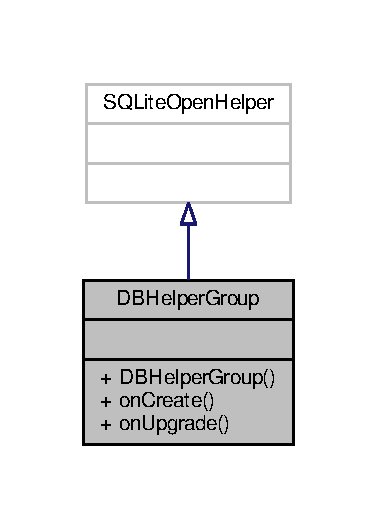
\includegraphics[scale = 1]{res/umlClasses/d_b_helper_group__coll__graph.pdf}
	\centering	
\end{figure}

\begin{figure}[H]
	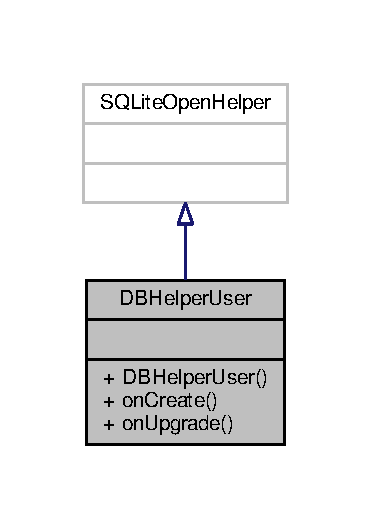
\includegraphics[scale = 1]{res/umlClasses/d_b_helper_user__coll__graph.pdf}
	\centering
\end{figure}

\begin{figure}[H]
	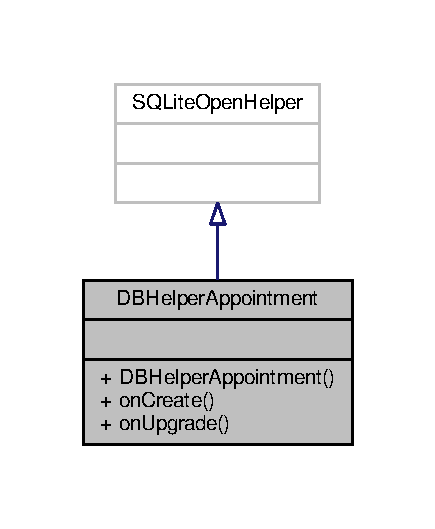
\includegraphics[scale = 1]{res/umlClasses/d_b_helper_appointment__coll__graph.pdf}
	\centering
\end{figure}

\begin{figure}[H]
	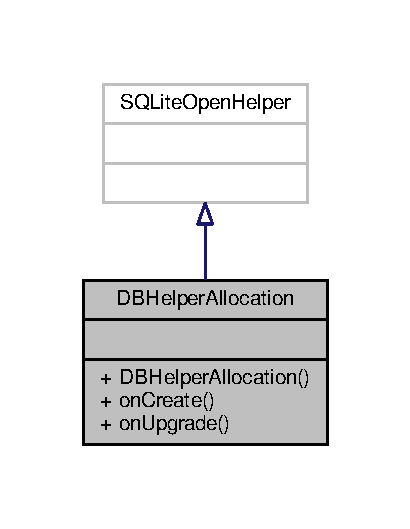
\includegraphics[scale = 1]{res/umlClasses/d_b_helper_allocation__coll__graph.pdf}
	\centering
\end{figure}



\textbf{FeedReaderContract}
\begin{figure}[H]
	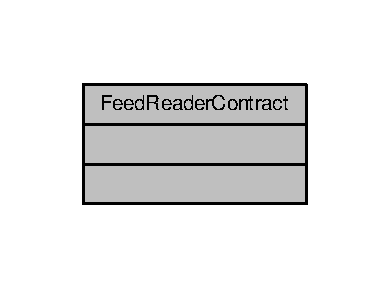
\includegraphics[scale = 1]{res/umlClasses/feed_reader_contract__coll__graph.pdf}
	\centering
\end{figure}
Die FeedReaderContract Klasse definiert in statischen Innenklassen wie die Tabellen der Datenbank aufgebaut sind. Jede der nachfolgenden FeedEntry Klassen implementiert dabei das interface BaseColumns.
CREATE ENTRIES erstellt dann aus den zuvor definierten Namen der Spalten die Tabelle in genau dieser Reihenfolge.
DELETE ENTRIES löscht die definierten Einträge wieder.

\textbf{FeedEntyGroup}
\begin{figure}[H]
	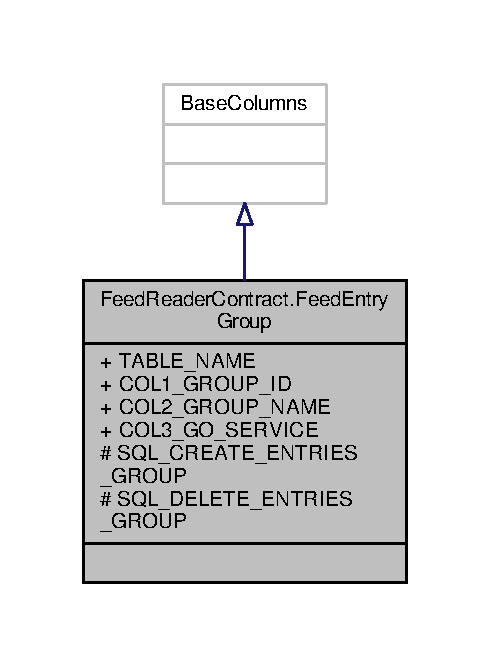
\includegraphics[scale = 1]{res/umlClasses/feed_reader_contract_group.pdf}
	\centering
\end{figure}
Die Innenklasse FeedEntryGroup definiert den Namen und die Spalten der Tabelle, welche die Gruppen auf dem Client speichert. 
Dabei steht in der ersten Spalte die eindeutige Gruppen ID (welche die Zeilen eindeutig unterscheidbar macht), in der zweiten Spalte der eindeutige Gruppenname und in der dritten Spalte, ob der GoService des aktuellen Benutzers für diese Gruppe aktiviert oder deaktiviert ist.
Wenn eine Gruppe gelöscht wird, dann wird auch ihr Eintrag in der Datenbank gelöscht.

\textbf{FeedEntyUser}
\begin{figure}[H]
	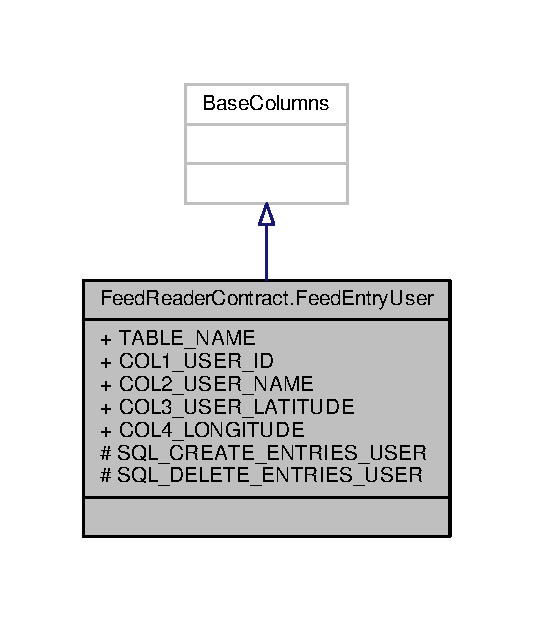
\includegraphics[scale = 1]{res/umlClasses/feed_reader_contract_user.pdf}
	\centering
\end{figure}
Die Innenklasse FeedEntryUser definiert den Namen und die Spalten der Tabelle, welche die Benutzer auf dem Client speichert. 
Dabei steht in der ersten Spalte die eindeutige Benutzer ID (welche die Zeilen eindeutig unterscheidbar macht), in der zweiten Spalte der Benutzername und in der dritten und vierten Spalte steht je ein Wert der zuletzt bekannten Gps Daten des jeweiligen Nutzers. 
Es werden nur Benutzer gespeichert mit denen der aktuelle Benutzer in mindestens einer gemeinsamen Gruppe ist.

\textbf{FeedEntyAppointment}
\begin{figure}[H]
	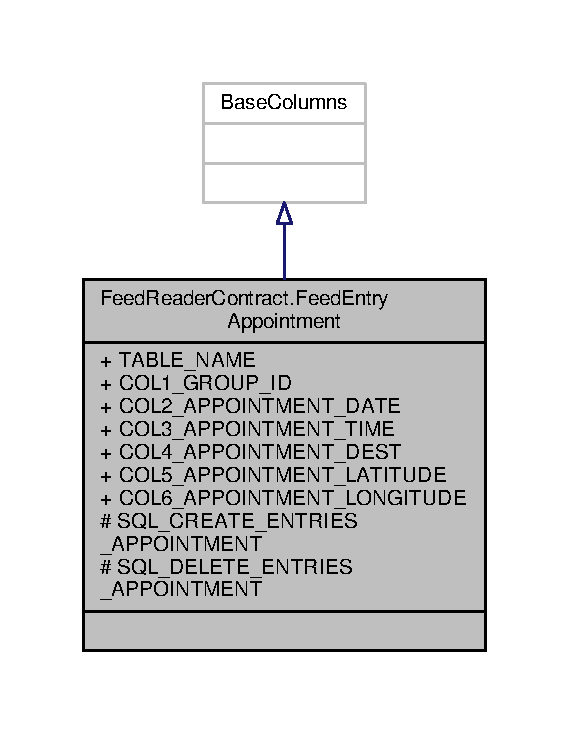
\includegraphics[scale = 1]{res/umlClasses/feed_reader_contract_appointment.pdf}
	\centering
\end{figure}
Die Innenklasse FeedEntryAppointment definiert den Namen und die Spalten der Tabelle, welche die Treffpunkte zu jeder Gruppe speichert. Jede Gruppe hat dabei nur eine Zeile, welche den Treffpunkt definiert. 
Dabei steht in der ersten Spalte die Gruppen id (welche die Zeilen eindeutig unterscheidbar macht), in der zweiten Spalte steht das Datum und in der dritten die Uhrzeit des Treffpunktes. In der vierten Spalte steht der Name des Zielortes und in der fünften und sechsten steht jeweils ein Wert der Gps Daten des Zielortes. 
Wenn sich der Treffpunkt der Gruppe ändert, dann werden die Werte des alten Treffpunktes überschrieben.
Sollte die die Gruppe des dazugehörigen Treffpunktes gelöscht werden, dann wird auch der Eintrag in dieser Tabelle gelöscht.

\textbf{FeedEntyAllocation}
\begin{figure}[H]
	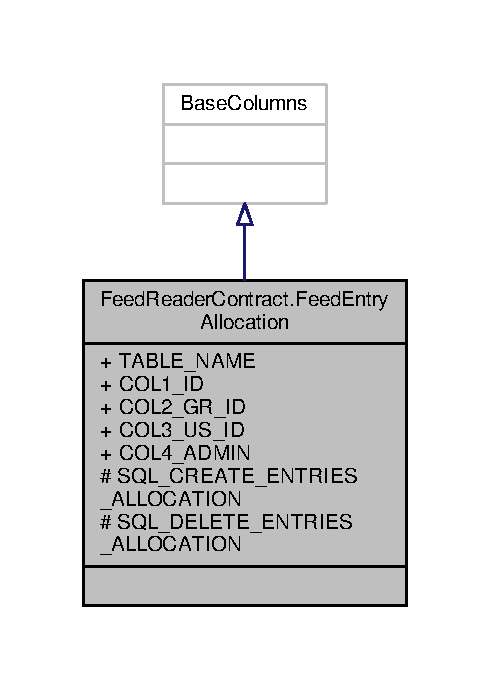
\includegraphics[scale = 1]{res/umlClasses/feed_reader_contract_allocation.pdf}
	\centering
\end{figure}
Die Innenklasse FeedEntryAllocation definiert den Namen und die Spalten der Tabelle, welche die jeweiligen Mitglieder jeder Gruppe speichert, in der der aktuelle Benutzer Mitglied ist. Zu jedem Mitglied wird vermerkt, ob dieses Administratorrechte hat.
Dabei steht in der ersten Spalte die Allocation id (welche die Zeilen eindeutig unterscheidbar macht und automatisch hochgezählt), in der zweiten Spalte steht die Gruppen id, in der dritten Spalte die Benutzer id und in der vierten Spalte, ob dieser Benutzer Gruppenadministrator ist oder nicht. 
Gruppen id wird für jedes Gruppenmitglied vermerkt, also kommt mehrmals vor, sobald mehr als ein Benutzer Mitglied dieser Gruppe ist. 

\paragraph{ObjectStructure}

\textbf{GroupClient}
Die Klasse GroupClient definiert wie eine Gruppe auf dem Client aufgebaut ist und welche Funktionalität ihr zur Verfügung steht.


\textbf{UserComponent}

\textbf{SimpleUser}

\textbf{UserDecorator}

\textbf{GroupAdmin}

\textbf{GroupMember}


\textbf{GoStatus}

\textbf{Link}

\textbf{GpsObject}


\textbf{Appointment}

\textbf{AppointmentDate}

\textbf{AppointmentDestination}








